\documentclass{article}
\usepackage[utf8]{inputenc}
\usepackage[a4paper, margin=2cm]{geometry}
\usepackage{multicol, caption}
\usepackage{authblk}
\usepackage[varg]{txfonts}
\usepackage{titlesec}
%\usepackage[T1]{fontenc}
%\usepackage{lmodern}
\usepackage[english]{babel}


\usepackage{amsmath}
\usepackage{amssymb}
\usepackage{amsfonts}
\usepackage{graphicx}% Include figure files
\usepackage{dcolumn}% Align table columns on decimal point
\usepackage{bm}% bold math
\usepackage{hyperref}% add hypertext capabilities
\usepackage{minted}
\usepackage[autostyle]{csquotes}

\usepackage[backend=biber,style=numeric]{biblatex}
\addbibresource{bib.bib}

\hyphenpenalty=10000
\exhyphenpenalty=10000

% CUSTOM FORMAT FOR SECTION
\titleformat{\section}[wrap]{\normalfont\bfseries}{\thesection.}{0.5em}{}
\titlespacing{\section}{12pc}{1.5ex plus .1ex minus .2ex}{1pc}
% CUSTOM SUBSECTION
\titleformat{\subsection}[wrap]{\normalfont\bfseries}{\thesubsection.}{0.5em}{}
\titlespacing{\subsection}{12pc}{1.5ex plus .1ex minus .2ex}{1pc}
% CUSTOM SUBSUBSECTION 
\titleformat{\subsubsection}[wrap]{\normalfont\bfseries}{\thesubsubsection.}{0.5em}{}
\titlespacing{\subsubsection}{12pc}{1.5ex plus .1ex minus .2ex}{1pc}

% CUSTOM LINE SPACING (Default 1.2 -> 1.2*1.25=1.5)
\linespread{1.25}

\newenvironment{Figure}
  {\par\medskip\noindent\minipage{\linewidth}}
  {\endminipage\par\medskip}

\title{PHYS6006 Final Report \\
       Magnetospheric structure associated with high-latitude auroras}
\author[1]{J. Plank}
\author[2]{R. C. Fear}
\affil[1, 2]{Department of Physics and Astronomy, University of Southampton}
\date{April 15, 2020}

\begin{document}
% TITLE BLOCK
\maketitle

% ABSTRACT
\begin{abstract}
    \noindent\textit{Context:} Only case studies have been done on the magnetospheric structure associated with the formation of high latitude aurora, and the connection of interplanetary magnetic field direction is suspected but has never been quantified.\\
    \textit{Aims:} To produce a statistical survey on the relationship between a northward pointing interplanetary magnetic field and a phenomenon known as transpolar arcs.\\
    \textit{Methods:} Using data from the ESA satellite Cluster, we analysed the ion temperature for many different values of $Z_{GSM}$, covering the plasma sheet as well as the magnetotail lobes.\\
    \textit{Results:} We found a direct link to IMF direction based on high temperature events observed in the lobe, suggesting high-latitude aurora form during periods of northward pointing IMF.
\end{abstract}

% SWITCH TO 2 COLUMNS
\begin{multicols}{2}

\section{INTRODUCTION}
Earth and the Sun are connected by more than just gravity, magnetic interactions between the two bodies are the cause of some of the most dramatic and complex phenomena on Earth. The most well known of these is the aurora (Borealis in the northern hemisphere and Australis in the southern). More commonly known as the northern and southern lights, these light shows come as a result of charged particles flowing along the Sun's magnetic field lines (known as solar wind) and making their way down to Earth in a zone known as the auroral oval \cite{AAAspaceweather}. The Sun's violent nature is also transmitted to Earth along its magnetic field, known as the `Interplanetary magnetic field` (IMF). This can result in satellite damage, radiation hazards to astronauts and airline passengers, telecommunications problems, and outages of power and electronics systems \cite{AAAspaceweather}.

The modern theory of the formation of the aurora was first proposed by Kristian Birkeland in 1903 \cite{birkeland2018norwegian}. He said that auroras are produced when solar wind encounters the geomagnetic field. The result of this is the formation of the plasmasphere in the equatorial plane of Earth's magnetic field \cite{cosmicelectrodyn}.

\subsection{Structure of Earth's magnetic field}
Figure \ref{fig:plasmasphere} is a representation of the solar-terrestrial environment. The solar wind, travelling with the interplanetary magnetic field from the sun \cite{Svalgaard_2010}, is coming from the left. It collides with the terrestrial magnetic field at supersonic speeds, creating a bow shock wave in front of the magnetosphere - the region where magnetic field lines connect to Earth at both ends - the boundary of the magnetosphere is the magnetopause. Supersonic solar winds compress at this boundary creating a magnetosheath between the magnetopause and the bow shock \cite{BSPP}.

\begin{Figure}
    \centering
    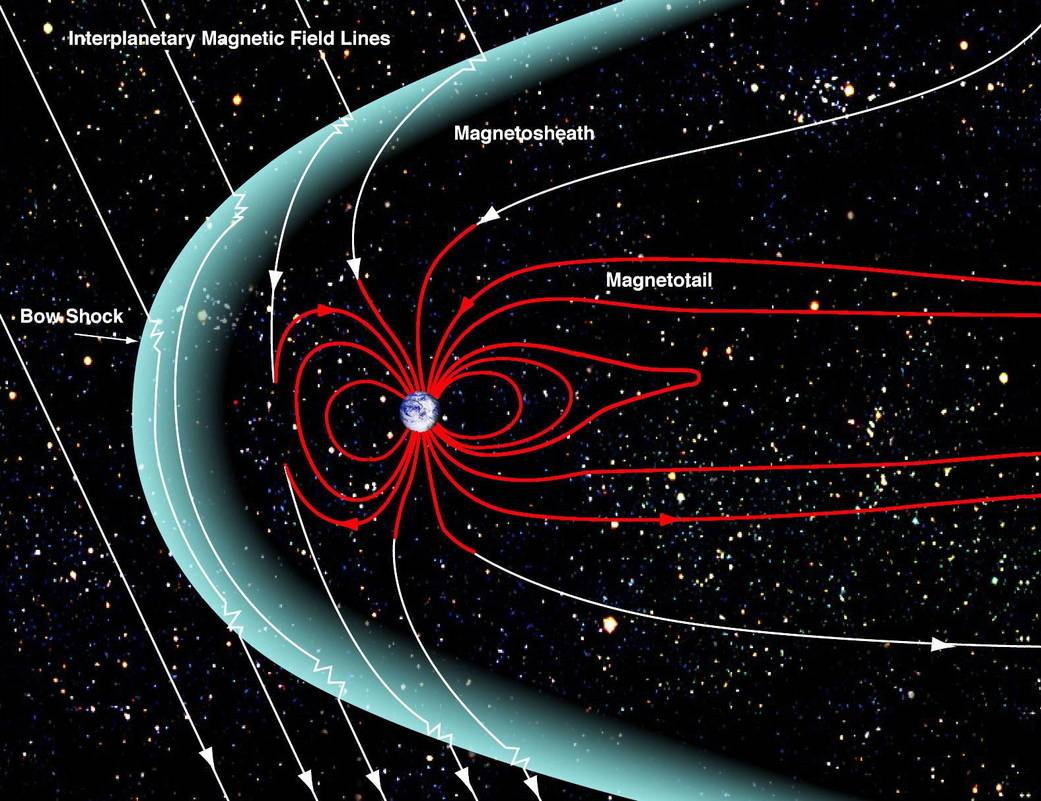
\includegraphics[width=0.8\linewidth]{NASA-Magnetosphere.jpeg}
    \captionof{figure}{Representation of the solar-terrestrial magnetic interaction. The sun is located to the left, producing solar winds and the IMF. Solar winds collide with the terrestrial magnetic field at supersonic speeds, creating a bow shock wave which encases the magnetosphere in a magnetosheath of compressed solar wind \cite{BSPP}. (Image courtesy of NASA)}
    \label{fig:plasmasphere}
\end{Figure}

Write more...


\section{OBSERVATIONS}
The majority of observations in this report come from Cluster, a group of four satellites built by ESA and launched in pairs on Soyuz rockets from Baikonur on the 16th July and 9th August 2000. They fly in a 57hr elliptical polar orbit and are arranged in a tetrahedron formation with a separation of between a few hundred and a few thousand km.

\subsection{Limitations of Cluster's orbit}
The orbit of cluster varies throughout the year. For significant portions of the year the satellite is well outside of the lobes, therefore the best months to extract data are July-October every year, where the spacecraft spends the majority of its time in the tail, and does not enter the magnetosheath. 

Figure \ref{fig:ClusterPos} shows Cluster's orbit through the month of September 2005 as an example, it does not cross the predicted magnetopause boundary (outer dotted parabola). Cluster will also cross through the plasmasphere in every orbit. This leaves the grey shaded region as the area of interest.

\begin{Figure}
    \centering
    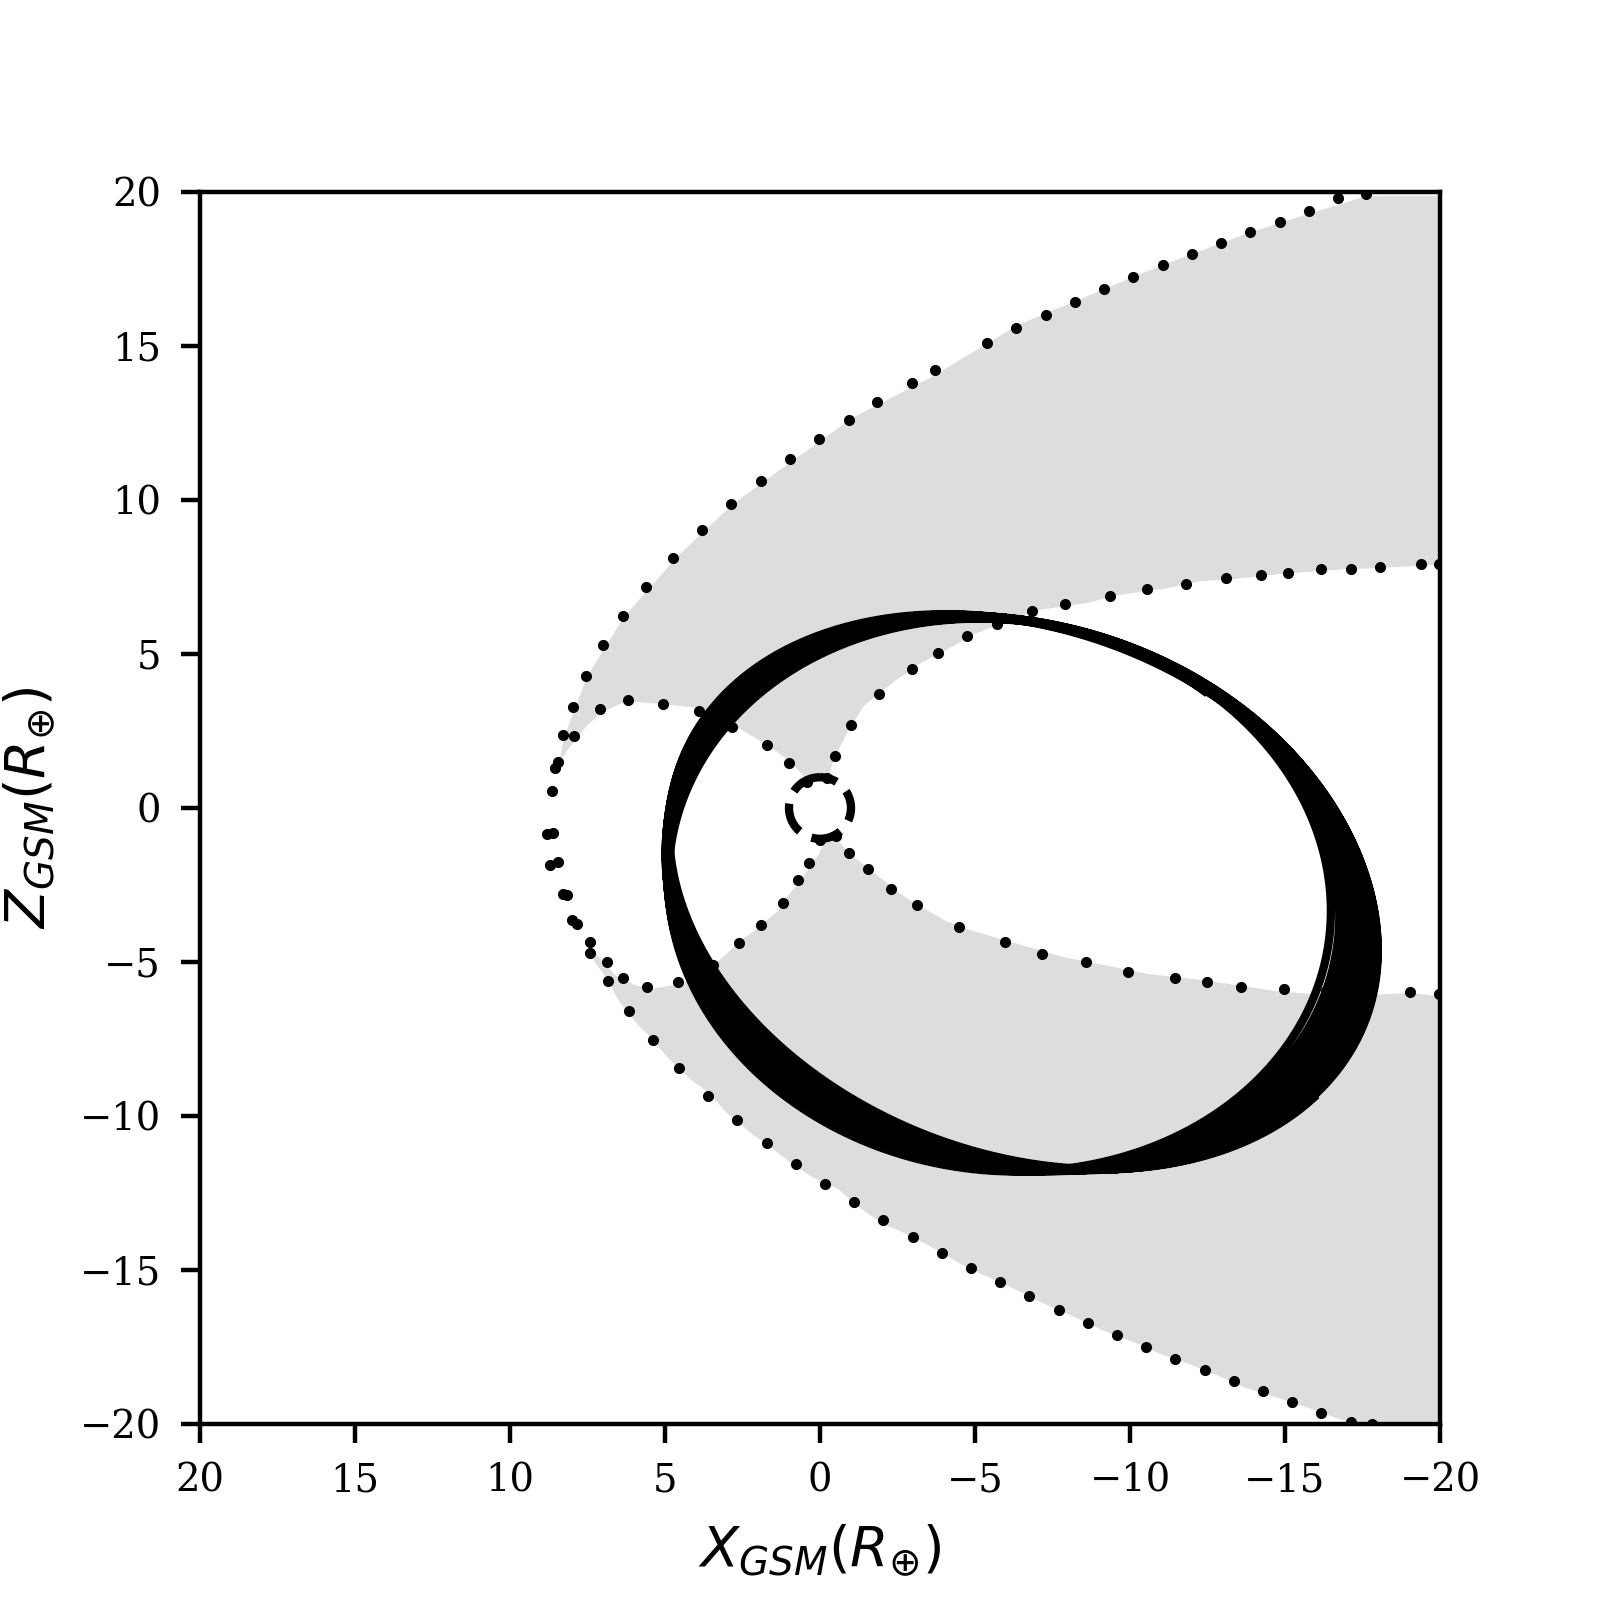
\includegraphics[width=0.75\linewidth]{sc_pos_09_05_coloured.png}
    \captionof{figure}{Plot of Cluster's orbit throughout September 2005 (solid), along with model results for the magnetopause and open-closed boundary on 15/09/2005 (dotted) \cite{Fear1506, substormConfModel}. The grey shaded region is of interest as it contains open field lines. If a reconnection event was detected while the spacecraft was in this region then it could indicate a transpolar arc. Plotting is done in the GSM coordinate system, where +X points to the sun and +Z points along the magnetic dipole axis.}
    \label{fig:ClusterPos}
\end{Figure}



\section{RESULTS}
HI

\section{DISCUSSION}
HI

\section{CONCLUSION: FUTURE WORK}
HI

\printbibliography
\end{multicols}
\end{document}